%TODO neues kapitel rechts starten

%\documentclass[xcolor = dvipsnames,11pt,a4paper,bibliography=totocnumbered,listof=totocnumbered]{scrartcl}
\documentclass[xcolor = dvipsnames,12pt,a4paper,bibliography=totocnumbered,listof=totocnumbered,twoside, letterpaper]{scrartcl}
\usepackage[english]{babel} %
\usepackage[utf8]{inputenc}

\usepackage[font={sf,footnotesize}, labelfont = bf]{caption}
\usepackage[font={sf,footnotesize}, labelfont = bf]{subcaption}
\usepackage{amsmath}
\usepackage{amsfonts}
\usepackage{amssymb}
\usepackage{mathtools} %neu wegen := Let  $ a \coloneqq  b $
\usepackage{graphicx} %
\usepackage{fancyhdr}
\usepackage{courier}
\usepackage{tabularx}
\usepackage{geometry}
\usepackage{setspace} % for title spacing etc.
\usepackage{multicol}
\usepackage{paracol}

%\usepackage{chngcntr1}
\counterwithin{figure}{section} % chapter-by-chapter figure caption

\usepackage{tabularx}
\usepackage[right]{eurosym}
\usepackage[printonlyused]{acronym}
%\usepackage{subfig}
\usepackage{float}
%\usepackage{floatflt} 
\usepackage[usenames,dvipsnames]{color}
\usepackage{colortbl}
\usepackage{paralist}
\usepackage{relsize} % set font size relative to others
%\usepackage{subcaption}
%\captionsetup{compatibility=false}
\usepackage{array}
\usepackage{blindtext}
%\usepackage{framed} 
%\usepackage{adjustbox} % breite von tables
\usepackage{xcolor} 
\colorlet{shadecolor}{gray!25}	
\usepackage{titlesec} % used for customizing chapter sections
\usepackage{parskip}
\usepackage{caption}
\usepackage[right]{eurosym}
%\usepackage{picins}
\usepackage[subfigure,titles]{tocloft}
\usepackage[pdfpagelabels=true]{hyperref}
\usepackage{listings}
\lstset{basicstyle=\footnotesize, captionpos=b, breaklines=true, showstringspaces=false, tabsize=2, frame=lines, numbers=left, numberstyle=\tiny, xleftmargin=2em, framexleftmargin=2em}
\makeatletter
\def\l@lstlisting#1#2{\@dottedtocline{1}{0em}{1em}{\hspace{1,5em} Lst. #1}{#2}}
\makeatother

\geometry{a4paper, top=27mm, left=30mm, right=30mm, bottom=35mm, headsep=10mm, footskip=12mm}

\hypersetup{unicode=false, pdftoolbar=true, pdfmenubar=true, pdffitwindow=false, pdfstartview={FitH},
	pdftitle={Scansify - A computation tool for designing customized on-body sensors},
	pdfauthor={Ba Thinh Tran},
	pdfsubject={Bachelor Thesis},
	pdfcreator={\LaTeX\ with package \flqq hyperref\frqq},
	pdfproducer={pdfTeX \the\pdftexversion.\pdftexrevision},
	pdfkeywords={Bachelor Thesis},
	pdfnewwindow=true,
	colorlinks=true,linkcolor=black,citecolor=black,filecolor=magenta,urlcolor=black}
%\pdfinfo{/CreationDate (D:20110620133321)}

\usepackage[
style= numeric,    % Zitierstil
isbn=false,                % ISBN nicht anzeigen, gleiches geht mit nahezu allen anderen Feldern
pagetracker=true,          % ebd. bei wiederholten Angaben (false=ausgeschaltet, page=Seite, spread=Doppelseite, true=automatisch)
maxbibnames=50,            % maximale Namen, die im Literaturverzeichnis angezeigt werden (ich wollte alle)
maxcitenames=3,            % maximale Namen, die im Text angezeigt werden, ab 4 wird u.a. nach den ersten Autor angezeigt
autocite=inline,           % regelt Aussehen für \autocite (inline=\parancite)
block=space,               % kleiner horizontaler Platz zwischen den Feldern
backref=false,              % Seiten anzeigen, auf denen die Referenz vorkommt
backrefstyle=three+,       % fasst Seiten zusammen, z.B. S. 2f, 6ff, 7-10
date=short,   % Datumsformat
firstinits=true,	%Vorname als Initialien
backend=bibtex,   
sorting=none,	% keine besondere Sortierung, sondern nach occurence          
]{biblatex}
\setlength{\bibitemsep}{1em}     % Abstand zwischen den Literaturangaben
\setlength{\bibhang}{2em}        % Einzug nach jeweils erster Zeile
\renewbibmacro{in:}{}

\bibliography{references}  % Bibtex-Datei wird schon in der Preambel eingebunden
\DeclareBibliographyCategory{cited}
\AtEveryCitekey{\addtocategory{cited}{\thefield{entrykey}}}

\newcommand\floor[1]{\lfloor#1\rfloor}
\newcommand\ceil[1]{\lceil#1\rceil}

\begin{document}

%\titlespacing{\section}{0pt}{12pt plus 4pt minus 2pt}{-6pt plus 2pt minus 2pt}
%\titlespacing{\section}{0pt}{12pt plus 4pt minus 2pt}{0.75 cm}

% Kopf- und Fusszeile
\renewcommand{\sectionmark}[1]{\markright{#1}}
\renewcommand{\leftmark}{\rightmark}
\pagestyle{fancy}
\lhead{}
\chead{}
\rhead{\thesection\space\contentsname}
%\lfoot{Lea Eckhart} %steht unten an seitenrand
\cfoot{}
\rfoot{\ \linebreak Page \thepage}
\renewcommand{\headrulewidth}{0.4pt}
\renewcommand{\footrulewidth}{0.4pt}

\fancyhf{} % clear all header and footers
%\renewcommand{\headrulewidth}{0pt} % remove the header rule
\fancyfoot[LE,RO]{\ \linebreak Page \thepage} % Left side on Even pages; Right side on Odd pages
\fancypagestyle{plain}{
  \fancyhf{}%
  \renewcommand{\headrulewidth}{0pt}%
  \fancyhf[lef,rof]{\ \linebreak Page \thepage}%
}


% Vorspann
\renewcommand{\thesection}{\Roman{section}}
\renewcommand{\theHsection}{\Roman{section}}
\pagenumbering{Roman}

% Commands

\newcommand{\newpara}{\\[0.125in]}
\newcommand{\sectionfix}{\vspace*{-1.5em} \thispagestyle{plain}}
\newcommand{\captionit}{\captionsetup{justification=centering,
labelfont=bf,textfont={normal}}}
\newcommand{\paragraphfix}{\hspace*{1.5em}}

% -------------------------------------------------------------
%
% Cover papers in front of main content
%
% -------------------------------------------------------------

%

%----------------------------------------------------------------------------------------------------------
%	Cover: includes all table of content etc...
% ----------------------------------------------------------------------------------------------------------
%

% ----------------------------------------------------------------------------------------------------------
% Titelseite
% ----------------------------------------------------------------------------------------------------------
\thispagestyle{empty}
\begin{center}
	
\includegraphics[scale=0.25]{pictures/hci_logo.png}\\
	%\vspace*{1.2cm}
		\vspace{1.2cm}
		SAARLAND UNIVERSITY \\
		Human Computer Interaction \\
		Departement of Computer Science\\
	\vspace{1.8cm}
	\textbf{Bachelor's Thesis}\\
	\vspace*{0.5cm}
	\Large
	\textbf{Scansify - A computation tool for designing customized on-body sensors}\\
	\vspace*{1cm}
	\large
	submitted by \\
	\vspace*{0.3cm}
	\textbf{Ba Thinh Tran} \\
	\vspace*{0.3cm}
	on MM DD, 2018	\\
	\vspace{1.8cm}
	\normalsize
	\newcolumntype{x}[1]{>{\raggedleft\arraybackslash\hspace{0pt}}p{#1}}
	\begin{tabular}{x{6cm}p{7.5cm}}
		\rule{0mm}{5ex}\textbf{Supervior:} & Prof.\ Dr.\ Jürgen Steimle \\  & \\
		\rule{0mm}{5ex}\textbf{Advisor:} & Aditya Shekhar Nittala, M.\ Sc.  \\ 
		\rule{0mm}{5ex}\textbf{Reviewers:} & Prof.\ Dr.\ Jürgen Steimle  \\ & Prof.\ Dr.\ Anonymous\\
	\end{tabular} 
	\medskip
%	\vspace{1.5cm}
%		Center for Bioinformatics \\
%		Saarland University \\
%		Bachelor’s Program in Bioinformatics
	\vspace{1cm}
	
\includegraphics[scale=0.18]{pictures/saarland_logo.png}\\
	%\includegraphics[scale=0.55]{Bilder/computerscience.png}\\
\end{center}
\pagebreak




% ----------------------------------------------------------------------------------------------------------
% Abstract
% ----------------------------------------------------------------------------------------------------------
%\setcounter{page}{1}
%\onehalfspacing
%\titlespacing{\section}{0pt}{12pt plus 4pt minus 2pt}{2pt plus 2pt minus 2pt}
%\rhead{KURZFASSUNG}
%\section{Kurzfassung}
%Lorem ipsum dolor sit amet, ...
%
%\vspace{-1,2em}
%\titlespacing{\section}{0pt}{12pt plus 4pt minus 2pt}{-6pt plus 2pt minus 2pt}
\thispagestyle{empty}
%\input{Chapters/Acknowledgment}
%\newpage
%\thispagestyle{empty}
%\mbox{}
%\newpage
%\thispagestyle{empty}
%\input{Chapters/Declaration}
%\newpage
%\thispagestyle{empty}
%\mbox{}
%\newpage
%\thispagestyle{empty}
%%-----------------------------------------------------
%
%    Content
%
%-----------------------------------------------------
\sectionfix
\section*{Abstract}
Recent advances in the HCI community have proven that on-body sensors changes the way we interact with our environment. By using our body, we obtain a better understanding on the correlation between perception and manipulation of the digital world. An initial exploration in this direction is the development of design tools for sensors. It helps maintaining the cost of fabrication and improves design iterations for better performance.\\
In this thesis, we propose a novel system (refered to as Scansify) for personalized design and rapid prototyping of thin-layered sensors. Using a low budget RBG-D camera, we were able to extract the finer details of the human body and enable the user to make annotations on top of its 3D model.\\
We provide design principles and detailed workflow description of the graphical user interface. Additionally, a user study is conducted to prove the feasibility and usability of the tool. Feedback in a semi-unstructured interview has been evaluated to obtain critical data for future iterations. Thereby, results illustrate that Scansify is a valuable tool for customized design processes of on-skin sensors.

%\newpage
%\thispagestyle{empty}
%\mbox{}
\newpage
%\pagebreak

% ----------------------------------------------------------------------------------------------------------
% Verzeichnisse
% ----------------------------------------------------------------------------------------------------------
% TODO Typ vor Nummer
\renewcommand{\cfttabpresnum}{Tab. }
\renewcommand{\cftfigpresnum}{Abb. }
\settowidth{\cfttabnumwidth}{Abb. 10\quad}
\settowidth{\cftfignumwidth}{Abb. 10\quad}
%
%\titlespacing{\section}{0pt}{12pt plus 4pt minus 2pt}{2pt plus 2pt minus 2pt}
%\singlespacing
%\rhead{Contents}
%\renewcommand{\contentsname}{Contents}
%\phantomsection
%\tableofcontents
%\pagebreak


\titlespacing{\section}{0pt}{12pt plus 4pt minus 2pt}{2pt plus 2pt minus 2pt}
\singlespacing
\rhead{Contents}
\renewcommand{\contentsname}{Contents}
\phantomsection
%\addcontentsline{toc}{section}{\texorpdfstring{Contents}{Contents}}
%\addtocounter{section}{1}
\addtocontents{toc}{\vspace{0.7cm}}
\addtocontents{lof}{\vspace{0.3cm}}

\tableofcontents

\clearpage

% ----------------------------------------------------------------------------------------------------------
% Abkürzungen
% ----------------------------------------------------------------------------------------------------------


\section{List of Abbreviations}
\begin{acronym}[OSGi] % längste Abkürzung steht in eckigen Klammern
	\setlength{\itemsep}{-\parsep} % geringerer Zeilenabstand
	\acro{OSGi}{Open Service Gateway initiative}
\end{acronym}
\newpage



% ----------------------------------------------------------------------------------------------------------
% Inhalt
% ----------------------------------------------------------------------------------------------------------
% Abstände Überschrift
%\titlespacing{\section}{0pt}{12pt plus 4pt minus 2pt}{-6pt plus 2pt minus 2pt}
\titlespacing{\section}{0pt}{12pt plus 4pt minus 2pt}{0.5cm}
%\titlespacing{\subsection}{0pt}{12pt plus 4pt minus 2pt}{-6pt plus 2pt minus 2pt}
\titlespacing{\subsection}{0pt}{12pt plus 4pt minus 2pt}{0.3cm}
%\titlespacing{\subsubsection}{0pt}{12pt plus 4pt minus 2pt}{-6pt plus 2pt minus 2pt}
\titlespacing{\subsubsection}{0pt}{12pt plus 4pt minus 2pt}{0.1cm}

\setcounter{secnumdepth}{4}
\setcounter{tocdepth}{1}

\titleformat{\paragraph}
{\normalfont\normalsize\bfseries}{\theparagraph}{1em}{}
\titlespacing*{\paragraph}
{0pt}{12pt plus 4pt minus 2pt}{0.1cm}

% header
\renewcommand{\sectionmark}[1]{\markright{#1}}
\renewcommand{\subsectionmark}[1]{}
\renewcommand{\subsubsectionmark}[1]{}
\lhead{Chapter \thesection}
\rhead{\rightmark}

\onehalfspacing
\renewcommand{\thesection}{\arabic{section}}
\renewcommand{\theHsection}{\arabic{section}}
\setcounter{section}{0}
\pagenumbering{arabic}
\setcounter{page}{1}


%----------------------------------------------------------------------------------------------------------
%	
%	Contents
% %----------------------------------------------------------------------------------------------------------




\titleformat{\section}[display]{\normalfont\Large\bfseries}{Chapter \thesection}{1.5em}{\Huge\bfseries }

\titlespacing{\section}
{0pt}{40pt}{45pt}{\phantomsection}
  
%%-----------------------------------------------------
%
%    Content
%
%-----------------------------------------------------


\sectionfix
\section{Introduction}
\label{sec:introduction}
Every day, we interact with the environment naturally through our skin. It happens in sports, while trying on clothes on a shopping trip or in other activities. Often, daily tasks become slowly overwhelming and there might not be a free hand available to decline an incoming phone call or unlock the car door.\newpara
Responding to a clear need to cope with this issue, research recently advances into the area of on-body interaction. Using modern electronics and data around us, devices for the skin have been developed to assist the users with their daily life activities (see \textbf{\autoref{fig:intro_sensors}}). The body can be used as an input surface to enable creative and distinct interaction possibilities e.g.\;accepting calls by touching the ear. In addition, the commonly known touch input can be extended with complex hand gestures which opens up more intuitive microactions such as pinching or rubbing.
Many of these projects aim to create an always-available, immediate and supportive technology that improves the way we engage in our environment. For instance, a visionary challenge is to equip the human body with a small processing sensor to facilitate direct access to a users' biomedical signals  \cite{Saponas:2009:EAI:1622176.1622208}. In an unforeseen car accident, the ambulance could immediately retrieve the medical documents from an unconscious victim by using his sensors. Furthermore, sensors can also be integrated as colorful overlays for the human skin which appeals to the aesthetics of body decorations e.g.\;sensors that look like tattoos \cite{Lo:2016:SDC:2901790.2901885, Kao:2016:DRP:2971763.2971777}.
\newpara
However, the fabrication methods of such sensors vary highly and can be rather costly since the size of a design overlay is often measured manually. The human body has unique properties, hence an analog recalibration procedure needs to be included for every new user. When mistakes happen during the fabrication, devices often have to be built from scratch again which can be expensive and time-consuming. Hereby, repetitive tasks often include positioning, scaling, copying or reorienting a 2D pattern on the body.

\begin{figure}[H]
    \captionit
    \centering
    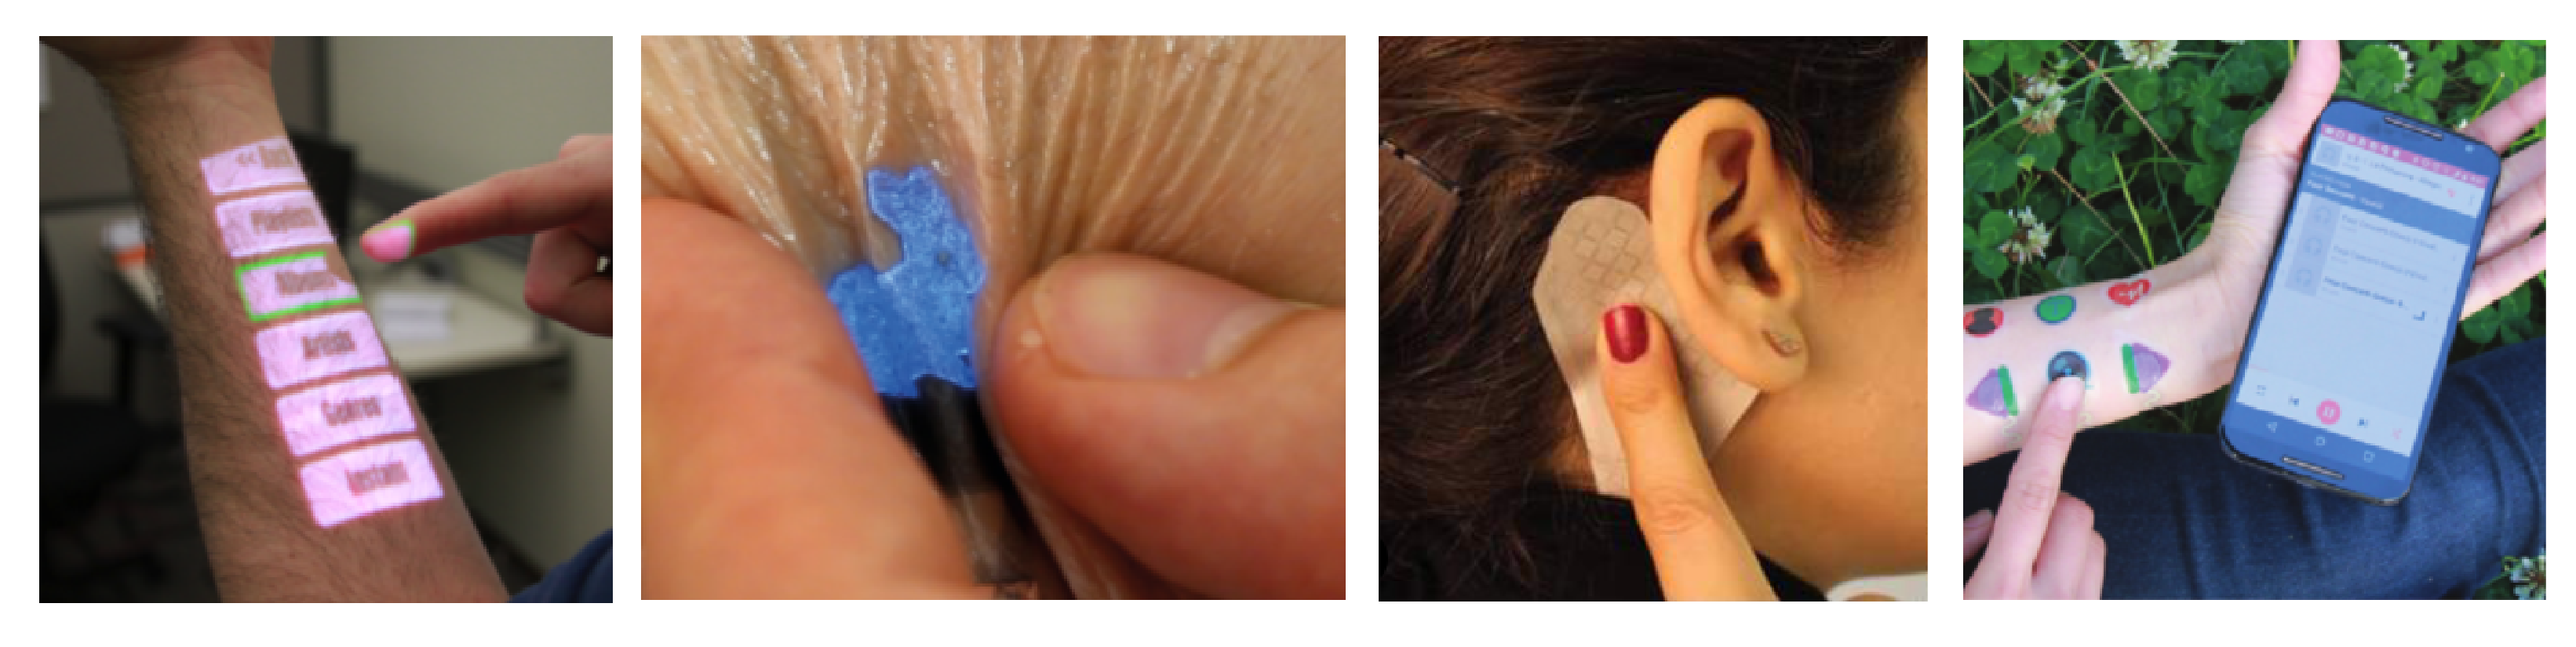
\includegraphics[scale=0.55]{pictures/onskin-01.png}
    \caption{An example of different on-skin interfaces. From left to right:\\ Omnitouch \cite{Harrison:2011:OWM:2047196.2047255}, SkinMarks \cite{Weigel:2017:SEI:3025453.3025704}, Multi-touch skin \cite{Nittala:2018:MST:3173574.3173607} and Skintillates \cite{Lo:2016:SDC:2901790.2901885}.
    }
    \label{fig:intro_sensors}
\end{figure}

As new forms of 3D printing and digital fabrication emerge, it is important to leverage automatized tools that are capable to ease this process for the user. In more detail, it is necessary to provide the ability to create designs that are easily replicable, shareable with others, archivable, fabricated remotely and adaptable to different bodies \cite{Gannon:2016:EOF:2858036.2858576}.\\
Additionally, there is a potential market to attract the audience - without technical background - to design and customize their own products. Such personalization is especially interesting for producing objects which adapt perfectly on a user's body such as braces, jewelry and other wearable devices.\newpara
Since the idea of producing touch sensors for the human skin is a rather recent discovery in human-computer interaction ( HCI ), very few design tools have been developed up to this day. 
It is hence important to introduce the first step towards the larger vision of easy customization and prototyping of on-body devices.

\subsection{Our approach}
We propose a digital design application (viz., Scansify) which enables users to create a design layout and then fabricate on-skin sensors \cite{Nittala:2018:MST:3173574.3173607} that conform to the user’s body. In our case, we have decided to focus on the arm part of the human body as it provides an easily accessible surface and is generally the most favorable area on the body for touch interfaces \cite{Harrison:2012:OIA:2148131.2148148, Harrison:2014:ILT:2598510.2598587}. Using a handheld depth sensor camera, our digital framework scans the outer form of the human figure and allows the user to digitally draw on the reconstructed model. After the drawing process, the input forwards into a post-processing pipeline and converts to a flat 2D shape which can be used for creating sensors (see \textbf{\autoref{subsec:overview}}).\\
After fabricating, the overlay wraps perfectly on the user's arm the way it was previously designed by the user (see \textbf{\autoref{fig:intro_tool}}).\\

\begin{figure}[H]
    \captionit
    \centering
    
\includegraphics[scale=0.65]{pictures/placeholder.png}
    \caption{An example of the work flow of Scansify.\\
    a) Drawing the layout in 3D;\\
    b) Our tool outputs a 2D shape which can be further processed;\\
    c) The shape fits perfectly on the skin
    }
    \label{fig:intro_tool}
\end{figure}

Scansify provides guidance, feedback, and support of various other operations. The following list summarizes the key implemented contribution of this thesis:\newpara
\label{item:functionality}
\textbf{Primary:} The core functionality
\begin{itemize} 
\item[\textbf{a)}] Capturing the human body with a RGB-D camera for acquiring precise geometry.
\item[\textbf{b)}] Live display of skin reconstruction process and depth stream from the camera.
\item[\textbf{c)}] Ability to annotate the digital body with a graphical user interface.
\item[\textbf{d)}] Unwrap algorithm that transforms the 3D drawing into a 2D shape.\\
\end{itemize}
\textbf{Secondary:} The remaining functionality that improves usability
\begin{itemize} 
\item[\textbf{e)}] Import and export of designs and 3d models.
\item[\textbf{f)}] Revert of latest change or completely reset the design.
\item[\textbf{g)}] Manipulation of camera view (steering, zooming or rotating).\newpara\\
\end{itemize}
Our approach especially target users that are not familiar with designing on-body sensors by providing an intuitive product for rapid prototyping. At the end, a use-case study is conducted and results are discussed to evaluate the feasibility and usability of the product. In addition, feedback is taken to refine the design principles for future iterations.
\subsection{Structure of the thesis}
The following list depicts a short overview of the subjects covered in the remaining chapters:
\paragraph*{\hyperref[sec:relatedwork]{Chapter 2}} presents recent work in on-body interaction and depth-sensing advances.
\paragraph*{\hyperref[sec:goals]{Chapter 3}} introduces the main concept and novel design considerations as a result of the related work chapter.
\paragraph*{\hyperref[sec:implementation]{Chapter 4}} illustrates a detailed workflow description of the graphical user interface and outlines the development process of Scansify.
\paragraph*{\hyperref[sec:results]{Chapter 5}} evaluates the results from a user study with respect to the feasibility and usability of our tool.
\paragraph*{\hyperref[sec:discussion]{Chapter 6}} concludes the thesis with a discussion on limitation and approaches for future work.

\newpage
\thispagestyle{empty}

%-----------------------------------------------------
%
%    Contents
%
%-----------------------------------------------------


\sectionfix
\section{Related Work}
\label{sec:relatedwork}
The HCI field of exploring the body as an input surface for possible interactions has been widely researched throughout the past years. Rapidly growing topics include the use of wearable systems, various sensing techniques and multi-touch input.\newpara
In this chapter, related work is discussed in the context of gestural 3D modeling, skin-based fabrication, and fabrication-aware design. The key ideas and limitations of the respective approaches are summarized at the end.
\subsection{On-Body Interaction}
\label{subsec:body}
The body is the most confidential and familiar interactive system to the human race.
The skeleton of a human arm affords a natural degree of freedom ( DOF ) offering a wide range of application possibilities \cite{Harrison:2012:OIA:2148131.2148148}. Additionally, interactions with the arm can always be accessible without the need for visual awareness to the target device \cite{Gustafson:2013:UPI:2470654.2466114}.
This always-available aspect combined with the unique context of using our body as a platform for access to communication and computation have proven to be a wide area of exploration \cite{Harrison:2011:OWM:2047196.2047255, Harrison:2010:SAB:1753326.1753394, Nittala:2018:MST:3173574.3173607, Dezfuli:2012:PIP:2325616.2325623, Gustafson:2011:IPL:2047196.2047233} and results received considerable attention in the HCI community.\newpara
Several papers focus their investigation on technical approaches for on-skin devices with touch-based capabilities. The research scope includes the use of capacitive sensing \cite{Kao:2016:DRP:2971763.2971777,Weigel:2015:IFS:2702123.2702391, Kao:2015:NFI:2702123.2702572}, on-body projection \cite{Harrison:2011:OWM:2047196.2047255, Harrison:2010:SAB:1753326.1753394, Xiao:2018:LOP:3173574.3173669}, ultrasound transmission \cite{Mujibiya:2013:STO:2512349.2512821}, magnetic \cite{Chan:2013:FPS:2501988.2502016} and electro-wave propagation \cite{Zhang:2016:SUB:2858036.2858082}. A particular interesting area is the use of optical devices to establish realistic touchable surfaces \cite{Harrison:2011:OWM:2047196.2047255}.\label{subsec:camera}
Hereby, researchers have advanced to augment physical context with the virtual modeling setting \cite{Leithinger:2011:DGI:2047196.2047268, Follmer:2012:KDR:2207676.2208403, Follmer:2010:CRP:1866218.1866230}. This trend aids novices to gain a more familiar feeling and hence incorporate a better understanding of the digital environment into their design \cite{Gannon:2015:TSA:2702123.2702581}.
A specific work by Andre D. Wilson \cite{Wilson:2010:UDC:1936652.1936665} investigates the application of depth-sensing cameras to identify touch input on a tabletop. Results illustrate that touch sensing is even possible on complex surfaces - such as concave or twisted regions - and allow a variety of unique interactions e.g.\;determine different hover states by measuring the distance between finger and target object.
One step ahead, Dezfuli et al.\cite{Dezfuli:2012:PIP:2325616.2325623}\;study in their paper ``\,PalmRC: Imaginary palm-based Remote Control for Eyes-free Television Interaction\," the possibilities of leveraging the palm as an interactive surface for TV remote control. They use an RGB-D camera - which is anchored on top of the television - to track gestural movements and identify distinctive tasks. A considerable benefit is that no calibration is required before sensing a palm of a different person. Each user presented with the device was able to immediately interact with the tool. However, both methods are restricted in their specific location area i.e.\;it was not possible to communicate with the system out of the cameras perception range. Our intention is to utilize the strength of the camera set-up to design a personalized sensor which the user can carry on the body. This provides the freedom of maximum mobility.
\newpara
Another important contribution, ``\,ExoSkin: On-Body Fabrication\," by Gannon et al.\;\cite{Gannon:2016:EOF:2858036.2858576} uses a custom built extruder to directly print on a drawn path which is projected onto the arm. Alternatively, the designed geometry can be exported and traditionally processed with a 3D printer and appropriate materials. However, the system uses a motion capture system which is considered costly to maintain. Authors stated that other tracking technologies should be considered such as the depth-sensing camera Kinect \cite{Zhang:2012:MKS:2225053.2225203}. Initial experimentation with the device resulted in a lack of accuracy. We anchor on this idea by utilizing the second generation version of Kinect which has a more reliable data stream than its predecessor \cite{wasenmuller2016comparison}.\\




Important in this context is the work ``\,Multi-Touch Skin: A Thin and Flexible Multi-Touch Sensor for On-Skin Input\," by Nittala et al.\,\cite{Nittala:2018:MST:3173574.3173607}. The group presents a novel fabrication approach for printing thin-layered mutual-capacitance-based touch sensors and is the first to achieve a high-resolution multi-touch capability (see \textbf{\autoref{fig_multitouch}}). Their fabricated overlay is able to withstand extreme deformations which can occur on local maxima of curvature, such as the wrists or similar joints. Furthermore, their study outcome scores in robustness, functionality and scalability and flags them as desirable features for future projects. However, authors stated that creating an input surface needs to consider the unique body properties such as the size.
Hence, a crucial requirement was the development of an interactive and intuitive design tool that can generate sensor layouts given any arbitrary 2D shape. The group stated that a limitation of the tool was the lack of a body measuring process and that subsequent work could include a scanning task into the existing pipeline. Our approach is tailored to this demand and provides a computer vision method to improve iterative design for on-skin devices.
Furthermore, Scansify creates a flatten 2D overlay that can be further processed to a thin-layered sensor as described above. Hence, our tool can be directly included as a preprocessing step for most projects.
\begin{figure}[H]
    \captionit
    \centering
    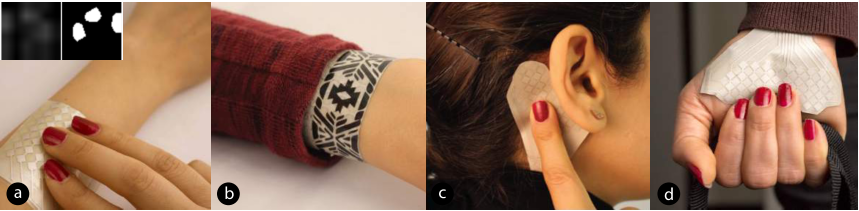
\includegraphics[scale=0.65]{pictures/multitouch.png}
    \caption{Multi-touch skin. Figure acquired from \cite{Nittala:2018:MST:3173574.3173607} \\
    a) multi-touch input on the forearm for remote interaction;\\
    b) aesthetic bracelet with multi-touch capabilities;\\
    c) input surface close to the ear for audio context;
    d) sensors for busy hands}
    \label{fig_multitouch}
\end{figure}
Lo et al.\;\cite{Lo:2016:SDC:2901790.2901885} introduce in
``\,Skintillates: Designing and Creating Epidermal Interactions\," a wearable technology using conductive silver ink on tattoo paper. The thin-layered sensors naturally wrap around the user's skin which, combined with the decorative design, facilitate an expressive and personal display. Application examples include capacitive buttons for mobile device control, body position detection and a light-emitting diode ( LED ) display that reacts to music. One of its fabrication challenges was to provide users, that do not have the technical knowledge for producing such devices, a sophisticated approach for flexible visual and electrical design. Therefore, the production cost of Skintillates was greatly reduced by integrating commonly available materials and easy-to-afford equipment. Still, the time consumption of building a specific device does highly vary with the design process of a tattoo pattern. The unique properties of a user's body make manually measuring the size of an arm a stagnant process. By importing our approach into their existing fabrication pipeline, it would enable a more flexible and rapid prototyping process for creating any personalized shape due to its capabilities on iterative design (see \textbf{\hyperref[item:functionality]{Chapter 1.1}})
. 
\newpara 
Recently, skin-friendly materials have been explored to replace the vastly expensive equipment to produce sensors. A successor to the approach of Skintilattes is ``\,DuoSkin: Rapidly Prototyping On-Skin User Interfaces Using Skin-Friendly Materials\," by Kao et al \cite{Kao:2016:DRP:2971763.2971777}. The group aims to make a durable on-skin circuitry available to non-experts in the HCI community by utilizing commodity materials. The device is able to sense touch input, to display an output and communicate wirelessly with other machines. Results from the user study show that the fabrication process was perceived ``\,fun and enjoyable\,". Furthermore, the ability to customize the devices with one's own design made it more intimate. Though, the design process uses paper stencils which limits the users in their customization experience. We share the same vision of providing users access to produce sensors without the demanding technical background. Furthermore, we believe that our tool can facilitate a faster and more individualistic approach to determine location and size of printed user interfaces. Scansify enables the users to draw any shape they desire and offers a flexible environment that encourages iterative rapid design.

\subsection{Design Tools in HCI for Fabrications}
The scientific contributions previously mentioned in \textbf{\autoref{subsec:body}} and \textbf{\autoref{subsec:camera}} have shown the demand for computational means to improve design iterations and sensor overlays for on-body interaction. Therefore, researchers have included external  graphics editor into their workflow e.g. Adobe Illustrator \cite{Kao:2016:DRP:2971763.2971777, Lo:2016:SDC:2901790.2901885}. However, the tools often lack flexibility and cannot be easily extendable in their own functionality. Hence, it is important to develop internal systems that are tailored specifically to personalized sensor modeling.\newpara
A novel approach is to engage the non-technical audience in advanced modeling with sketch-based 2D drawings \cite{Johnson:2012:SMS:2212776.2212390, Saul:2010:SAC:1935701.1935717}. One such system even incorporates the user to design and fabricate on the material itself \cite{Willis:2010:IFN:1935701.1935716, }. Based on a similar idea, ``\,Tactum: A Skin-Centric Approach to Digital Design and Fabrication\," by Gannon et al. \cite{Gannon:2015:TSA:2702123.2702581}\;presents a system to directly use the skin as the design interface. Tactum allows non-experts to intuitively create precise forms on top of the human body by capturing different gestures e.g.\;touch, grab, drag and rub. The implementation relies on a single depth camera that senses the input on the body. Additionally, a monitor is mounted on the desk to visualize a 3D representation of the arm and the drawn artwork on it (see \textbf{\autoref{fig:tactum_sub1}}). Results reveal that both experts and non-experts were enthusiastic about the system and further research could stabilize the feasibility of the project. The overly simplified representation of the arm was considered too coarse and was a highlighted limitation (see \textbf{\autoref{fig:tacum_sub2}}). It was suggested to portray the geometry of the arm and its texture more precisely to convey a more steady bridge between interaction and manipulation. Our work aims to investigate this idea further by digitally reconstructing the finer details of a human body through a depth stream.
\begin{figure}[H]
\centering
\captionit
\begin{subfigure}{.5\textwidth}
  \centering
  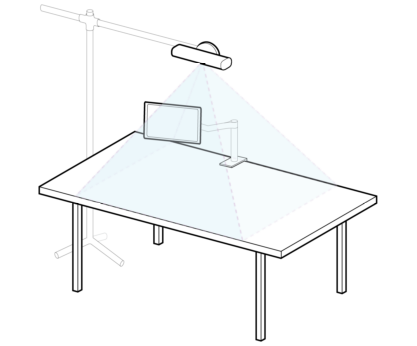
\includegraphics[width=.6\linewidth]{pictures/tactum_1}
  \caption{An illustrative drawing of the setup: The arm would be scanned on the desk}
  \label{fig:tactum_sub1}
\end{subfigure}%
\begin{subfigure}{.5\textwidth}
  \centering
  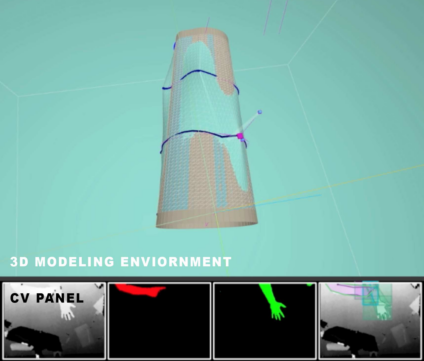
\includegraphics[width=.6\linewidth]{pictures/tactum_2}
  \caption{The design environment:\\3D model is live updated}
  \label{fig:tacum_sub2}
\end{subfigure}
\caption{Tactum. Figure acquired from \cite{Gannon:2015:TSA:2702123.2702581}}
\label{fig:tactum}
\end{figure}
\subsection{Summary}
This chapter presented an overview on the current vision and limitations of on-body interaction in the context of sensor design. In the past years, several researchers have explored the possibilities of sensing techniques and sensor capabilities. The wide range of investigation can include using different materials \cite{Lo:2016:SDC:2901790.2901885}, external tools \cite{Gannon:2016:EOF:2858036.2858576} or exploring different interaction possibilities \cite{Harrison:2012:OIA:2148131.2148148}. Still, these works often suffer from inprecise arm geometry acquisition \cite{ Gannon:2015:TSA:2702123.2702581}, lack of customization capability \cite{Kao:2016:DRP:2971763.2971777} or inflexibility from third-party drawing tools \cite{Kao:2016:DRP:2971763.2971777, Lo:2016:SDC:2901790.2901885}. Hence, an upcoming challenge and philosophy is to introduce intuitive fabrication methods that assists the user in building their own customized sensors. These works - including ours - depict an initial investigation on skin-centric design approaches. In the next chapter, ideas and findings from this scientific research are used to facilitate design recommendations for our tool and to overcome the prior mentioned limitations.

\newpage
\pagebreak
%
%-----------------------------------------------------
%
%    Contents
%
%-----------------------------------------------------

\sectionfix
\section{Design Goals}
\label{sec:goals}
This chapter describes the goal of our design tool and briefly outlines the design considerations. Additionally, we present an architectural pipeline on how we achieved this task. 
\subsection{Requirements}
Advances in research have shown that worn electronics and sensors can enable the human body to be more interactive in context of how we complete daily and complex tasks in an efficient way \cite{Amft:2008:RDA:1343127.1343441}. While the technology constantly evolves around optimizing and building novel sensors, there are still challenges to be considered in regards to the fabrication process and its resulting costs. Our idea is to put upon the research domain of computer graphics and human-computer interaction to ease the aforementioned process by providing the user a graphical interface for designing their own on-body sensors. The tool is required to be guiding the user through its main functionality, provide fast iterable setup and be able to support multiple body locations and users. Our software prototype pursues these six following requirements.
\raggedbottom
\paragraph*{Rapid Prototyping}
\begin{description}
\item[R1] Allow the user to apply design ideas quickly within the system
\item[R2] Provide a fast iterative workflow
\item[R3] Maintain an easy to use interface
\item[R4] Offer a system that can be set-up effortlessly
\end{description}

\paragraph*{Flexible Scalability \& Design}  
\begin{description}
\item[R5] Must be applicable to multiple locations on the arm
\item[R6] Must be applicable to all users \\[3.25ex]
\end{description}

While the design and fabrication process of sensors is rather common nowadays, it raises a number of challenges to people that do not have the required technical background to produce sensors for their own uses. The design tool is therefore inclined to fit users that do not have that expertise but want to have their own sensor design fabricated rapidely. This aspect is summarized in \textbf{R1}. When asked to design specific images, many people are not confident in their own skills and will hence be hesitant about it \cite{Dixon:2010:IUS:1753326.1753459}. Therefore, many drawing softwares offer the flexibility to import existing templates into the tool \cite{Iarussi:2013:DAA:2501988.2501997, Fernquist:2011:SRE:2047196.2047245}. This creates an initial starting point for the users and helps them to be more creative with their own work which leads to our second requirement \textbf{R2}. On the other hand, \textbf{R3} is based on the consensus that an intuitive interface also directly accelerate the work flow of the process itself and improves the user experience \cite{Hassenzahl:2008:UET:1512714.1512717}. This criteria is a must-have for any interfaces targeting users without advanced knowledge of such tools.\\ Camera-based systems are often used in research domain to model environments in real dimensions, track movements or identify objects. However, there are a lot of products that are expensive since they are dependant on several cameras, large areas, certain lighting conditions or multiple people to set up \cite{Rahimian:2015:OCP:2821592.2821596, Dezfuli:2012:PIP:2325616.2325623}. \textbf{R4} targets these problems for users that do not have the resources mentioned above.\\Regarding the scalability, the core idea behind \textbf{R5} is to provide the user a feeling of intimate customization during the design process \cite{Kao:2016:DRP:2971763.2971777} while \textbf{R6} focuses on the fact that anyone should be able to use the software regardless of their unique body size \cite{Nittala:2018:MST:3173574.3173607, Dezfuli:2012:PIP:2325616.2325623}.\newpara
In this section, we have presented a list of requirements which aligns with our vision of a personalized fabrication process for on-body sensors. Following, we will discuss the demanding challenges and open research questions that existed during our work and realization of the previously mentioned points.
\subsection{Challenges}
We came across multiple technical difficulties during our research on how we wanted to achieve this goal. 
\paragraph*{Digital Model Acquisition} The human anatomy is a widespread topic. 
Each human's body is as unique as one's own fingerprint. Properties such as skin color, skin elasticity, size and irregularities on the body define our individual characteristics \cite{Nittala:2018:MST:3173574.3173607}. Capturing all of those unique attributes is a prominent research challenge in computer vision. A solution to this problem is the use of a camera-based scanning and reconstruction method which is able to leverage most of these properties. This approach is ideal for complex geometries that require a massive amount of data for an accurate description of its surface \cite{Gopi:2002:FEP:646016.678279}. The acquisition initially creates point clouds of data from the outer form of the object. Afterwards, the resulting information allows us to digitally capture the exact size and shape of the physical object into the computer as a digital 3-dimensional ( 3D ) representation e.g. a body part in virtual environment. At last, post-processing methods are applied to the dataset which can include fixing holes, filtering noises or classification \cite{Weyrich:2004:PSS:2386332.2386347} to finalize the reconstruction.\\
A number of digital models of body parts can also be acquired by capturing mid-air gestures and a search through populated databases \cite{Holz:2011:DMI:1978942.1979060}. However, these geometries vary massively in their resolutions and will therefore not provide an idealized model for personalized design.
\newpara
As previously mentioned in the related work, we will focus on the reconstruction of the human arm as it offers the most comfortable surface for touch input and gives the best haptic feedback to the users \cite{Harrison:2014:ILT:2598510.2598587, Weigel:2014:MTU:2556288.2557239}. Remarkably, hands were also highly rated among the study participants but because of its joints and complex non-flat surface it was rather hard to interact with. The form of the forearm was more straight forward and aligned to a flat touchpad commonly known in laptops.
\paragraph*{Camera Parametrization}
A 3D scan can either be a result of a simple RGB-D camera \cite{Wilson:2010:UDC:1936652.1936665, Dezfuli:2012:PIP:2325616.2325623} or a complex motion-capture technology \cite{Gannon:2016:EOF:2858036.2858576}. Both setups have their own benefits and drawbacks. The RGB-D camera is reliant on a more software-oriented process to retrieve the depth information of the device and to reconstruct a 3d model. Depending on the cost of the software, this approach can be very cost efficient and fast to set up. On the other hand, a mocap system is rather expensive nowadays since it uses a lot of cameras to capture different angles. Furthermore, it is usually restricted to a certain room space which might not always be available. However, the results can be worth the time and money since it provides a more realistic image of the scenery which is important for particular application domains e.g. animations in movies.\newpara
In our case, we decided to use the motion-sensing device Kinect (2nd generation) which is produced by Microsoft. Kinect contains an RGB camera, a depth sensor, an IR emitter and a multi-array microphone (see \textbf{\autoref{fig:kinect}}).\newpara
\begin{figure}[H]
    \centering
    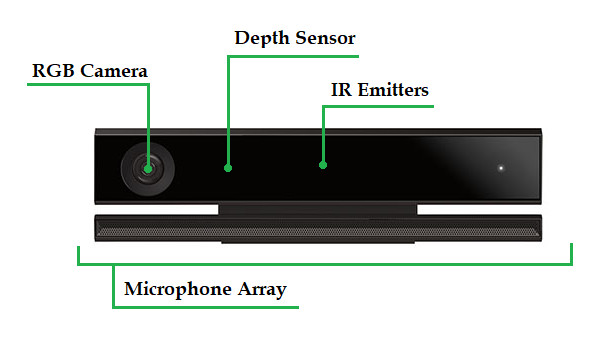
\includegraphics[scale=0.7]{pictures/kinect.png}
    \caption{Architecture of 2nd generation Kinect}
    \label{fig:kinect}
\end{figure}
By emitting light signals and then measuring how long it takes them to return, Kinect is able to differentiate light reflecting from objects in a room and therefore provide an accurate depth estimation. This technology is referred to as the \textit{time-of-flight} ( TOF ) method \cite{lachat2015first, sell2014xbox}. Due to its affordable price compared to most of the 3D scanners on the market, many researchers and private consumers are using the Kinect as a tool for tracking the human body \cite{Harrison:2011:OWM:2047196.2047255, Dezfuli:2012:PIP:2325616.2325623, Wilson:2010:UDC:1936652.1936665}. Additionally, the second version of its product line obtains much better resolution while also reducing noises and interferences from outside IR sources \cite{wasenmuller2016comparison}.\\
With the capability of its SDK, we are able to use the Kinect as a low-cost handheld sensor to scan different parts of an object and work with its resulting organized point clouds.

\paragraph*{Design Environment}
As previously mentioned in the related work, digital design tool has been developed for various hybrid applications in fabrication. Most of the work has been focusing on using the skin as an interactive surface for gestural or machine input. These digital fabrication approaches enable non-experts to intuitively create precise shapes on top of complex physical surroundings. While these technologies open up a large design space for users without the technical background to the fabrication process, there is not yet a pipeline that connects the design process with a higher level user interface. This approach gives the user more flexibility in their creative customization process and yields a good balance between rapid prototyping and sophisticated design on a representational model.\\
Using a digital process also enables us to translate existing analog methods into a more computational workflow. Manipulating patterns like scaling, positioning, duplicating and reorienting is a time-consuming task in the real world but is easily integrated into our tool. Sharing your own designs with multiple users is another benefit. It enables others to review your work and contribute to it which in return improves the product. Furthermore, design process often happens simultaneously with a lot of different iterations before committing to an end result. The capability to visualize a current prototype vastly improves the design-to-production workflow and can offer a much broader control over the final outcome. At last, a user interface provides a natural mean to guide the user and give him feedback on its current iteration. This user-centric approach helps every user to build their own sensors without consuming too much time on the process itself. In combination with the Kinect, the design environment offers an initial easy-to-setup and cheap approach for customized sensor designs.

\subsection{Overview}
\label{subsec:overview}
The goal of this work is to allow the user to create a flatten 3D shape of a body part for personalized on-body sensors using the RGB-D camera Kinect and our design tool. Therewith, the rigid volumetric representation of an arm is reconstructed and further processed for display to the user. Unlike to related work, this approach highly focuses on the precise geometry acquisition of the scanned object and on the flexibility of the tool for rapid prototyping. A pipeline overview of the sequential steps performed for each depth frame is depicted in \textbf{\autoref{fig:pipeline}}. Some of the algorithms listed in this part are tailored to the existing approaches of KinectFusion \cite{Izadi:2011:KRR:2047196.2047270} which will be discussed profoundly in \autoref{sec:implementation}.\newpara

\begin{figure}[ht]
    \centering
  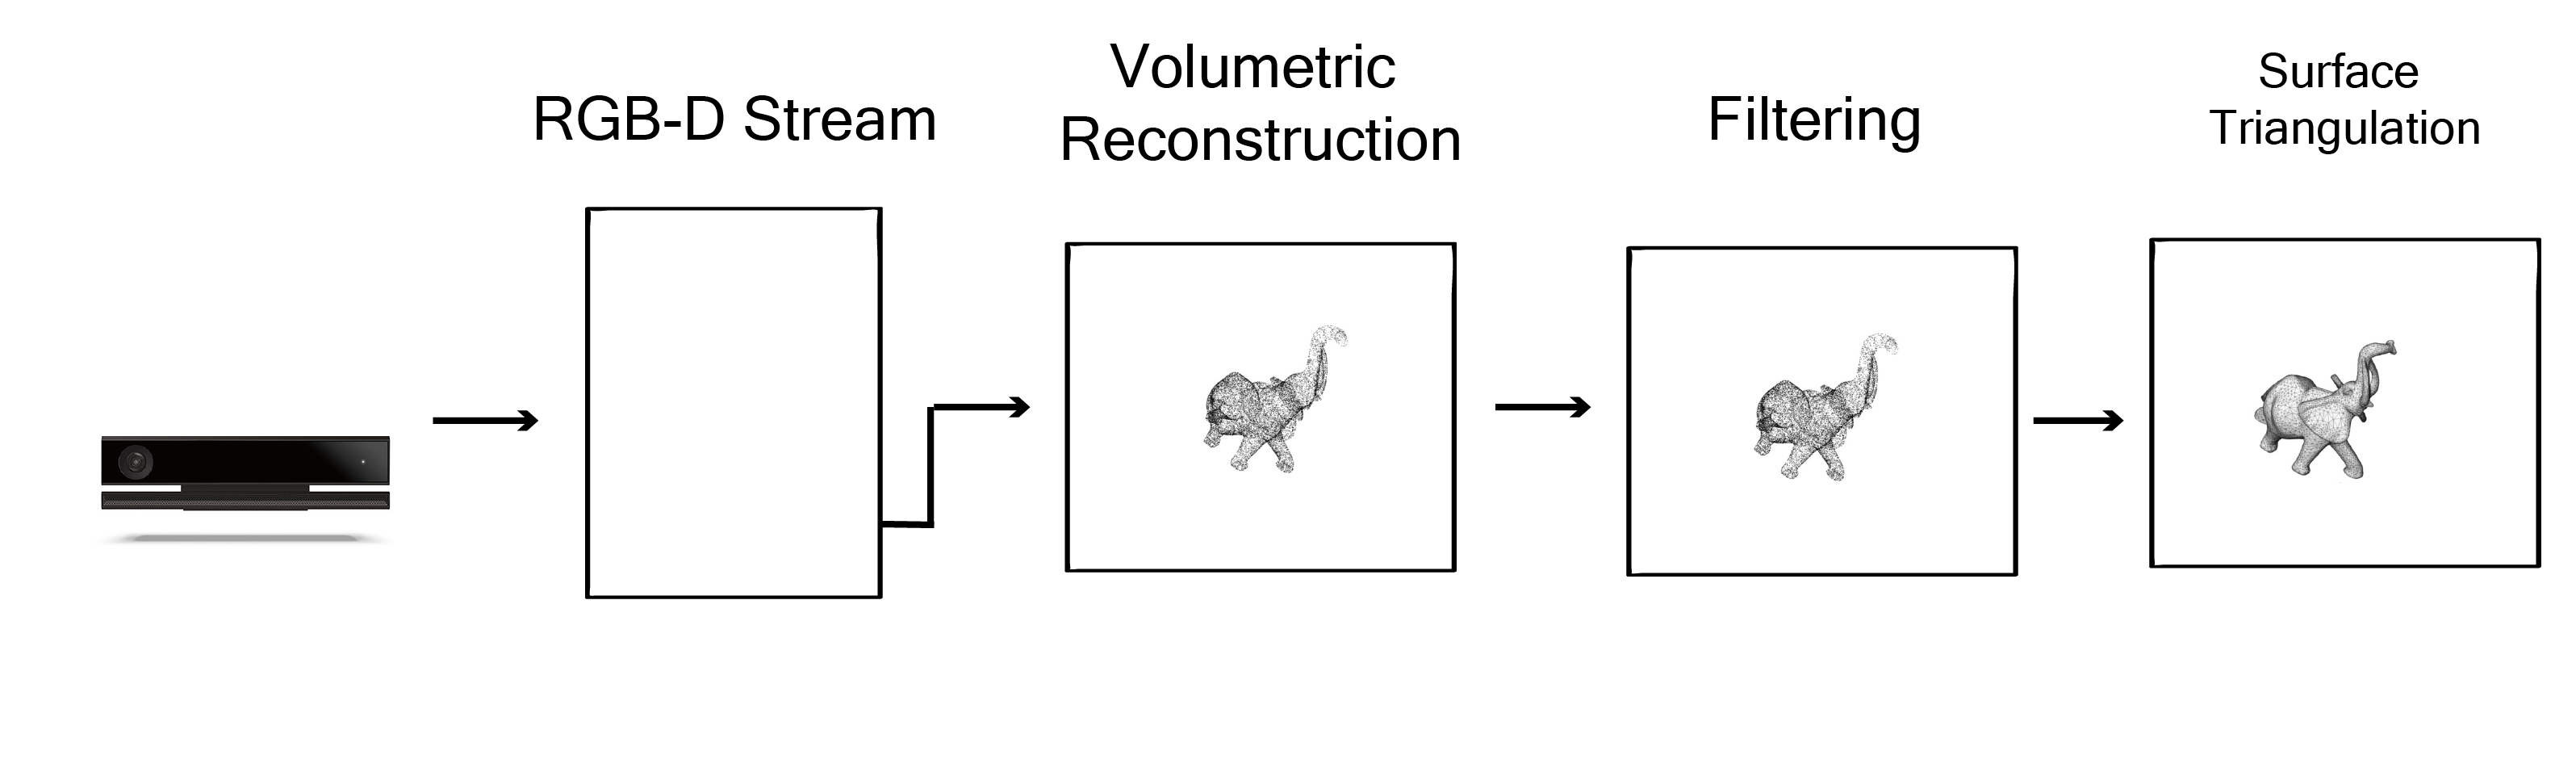
\includegraphics[scale=0.55]{pictures/pipeline_core}
    \caption{An architectural overview illustrating how raw data from the Kinect is processed to a water-tight model.}
    \label{fig:pipeline}
\end{figure}

Initially, the system continually tracks the camera pose and uses an iterative closest point ( ICP ) approach to join the live depth data into a geometrically precise 3D model of the room in real time (see \textbf{\autoref{fig:icp}}). Hereby, the camera can either be rotated around the arm or the arm itself can turn around its axis in front of the camera as long as every part is being exposed to the camera lens for a fraction of a second. Even small movements, which could be caused by a minor shake, results in a new viewport of the scene and can be used to improve the model i.e. similar to a \textit{supersampling} effect \cite{Damera-Venkata:2009:DS:1477926.1477935}.\\
\begin{figure}[ht]
    \centering
  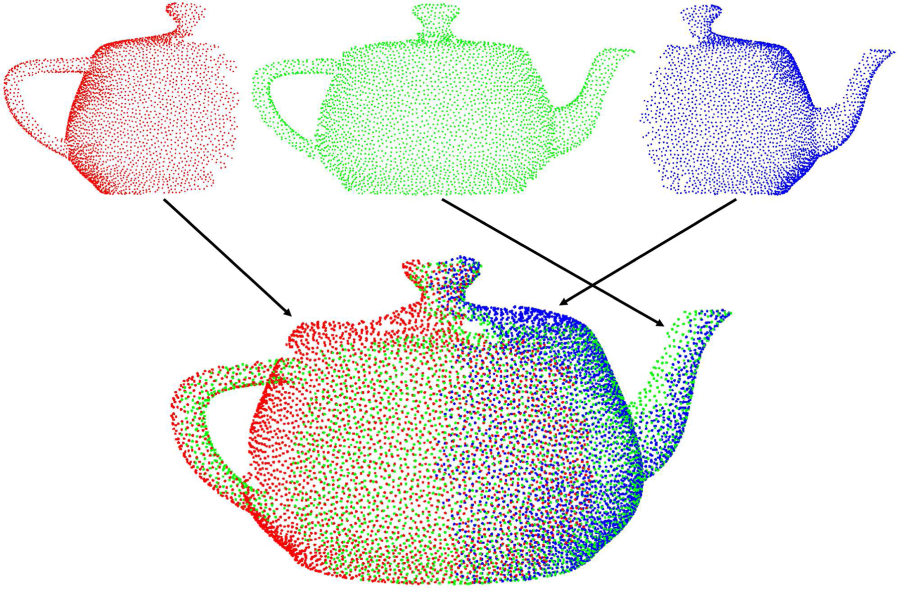
\includegraphics[scale=0.45]{pictures/icp}
    \caption{An illustration of the ICP algorithm. Multiple different views of the same object are taken iteratively to construct an overall completed model by aligning similiar features. Figure acquired from \cite{kwok2016improvements} }
    \label{fig:icp}
\end{figure}
Moving forward, several filtering methods are applied to the data set to remove background and outliers. A volumetric surface representation \cite{Curless:1996:VMB:237170.237269} is applied to the oriented point clouds which result in a continuously updated voxel grid wherein each cell stores its assumed distance to the physical surface. This surface triangulation works efficiently on the noisy data from the Kinect by filling holes and adapting to sensor motion.\\
The model then transfers to the raytracing pipeline which results in several rendered images taking physical properties into account e.g. lights and reflections. Multiple components for building an efficient acceleration structure, tree traversal and shader are asynchronously parallelized (ref sub-chapter).\\
Afterward, the user has the ability to manipulate the environment of the computated object. Each change - be it camera angle or annotations on the object - will return to the raytracing pipeline as a request for an updated image. This exchange lapses in a continuous feedback loop and will only end when the user resets the model.\\
At last, the generated drawing is extracted and the data evaluates to a coherent graph. All vertices and edges flatten from a 3D perspective into a 2D plane in SVG format (ref sub-chapter).\\
The finished shape can be further used in a postprocessing pipeline to initiate the fabrication process for a multi-touch sensor \cite{Nittala:2018:MST:3173574.3173607}.

\newpage
\pagebreak
%

%-----------------------------------------------------
%
%    Contents
%
%-----------------------------------------------------

\sectionfix
\section{Implementation}
\label{sec:implementation}
\subsection{Work flow}
\begin{itemize}
\item GUI
\item Detailed step-by-step manual on how to use the application
\item tailored to the methods chapter mentioned above
\end{itemize}
\subsection{Dependencies}
A great benefit of Scansify is that it does not rely onto any major image processing library like openGL or PCL but rather makes use of the native implementation framework KinectFusion \cite{Izadi:2011:KRR:2047196.2047270}. 
\subsubsection{Kinect Fusion}
This framework allows users to create high-quality 3D reconstructions of indoor rooms in real-time by moving the Kinect around the scene. The core system provides a great amount of utilities which we uses to achieve our goal. Unfortunately, they only provide us with an api structure which imposes a restriction on the use of their source code. Partiularly, our pipeline extends their implementation of a shader and surface reconstruction.
The function of these components and how we integrated them into our project will be enlighten in more detail in the respective paragraph later on.
\subsection{Kinect Fusion}
\begin{itemize}
\item Introduction
\begin{itemize}
\item system allows a user to pickup a standard Kinect camera and move rapidly within a room to reconstruct a high-quality, geometrically precise 3D model of the scene
\item avoids the reliance on RGB allowing use in in- door spaces with variable lighting conditions
\item reconstructing surfaces, which more accurately approximate real-world geometry
\item aim to perform camera track- ing without the need for prior augmentation of the space
\end{itemize}
\item What do we use
\item remark regarding restricted source code access
\item tailored approach
\end{itemize}
\subsection{Software architecture}
The software pipeline described in the previous chapter (see \autoref{subsec:overview}) was implemented as a Microsoft Foundation Classes ( MFC ) application and written in C++. MFC is a collection of frameworks created by Microsoft for programming systems with graphical user interfaces \cite{Fayad:1997:OAF:262793.262798}. The purpose of the different modules are explicitely explained in \autoref{sec:goals}. Therefore, following exempt will rather give an outlook on how these components interact with each other and how they were realized.
\subsubsection{Data processing}
The depth stream is collected via the Kinect software development kit ( SDK ) which is the official programming library for processing raw input from the Kinect \cite{Abhijit:2012:KWS:2490784}. Hereby, data is presented as numerical values that needs to be mapped to the real world coordinates. Since the point cloud scan is quite noisy initially, a conditional and outlier filter technique is applied to improve more smooth and accurate data aquisition. These methods essentially remove extreme points that are behaving extraordinary due to their position in relation to their neighbours.\\
Afterwards, multiple point clouds are merged together by using advanced volumetric representation \cite{Curless:1996:VMB:237170.237269} and ICP which is provided by Kinect Fusion.
\subsubsection{Rendering}
A major challenge was the optimization of our rendering pipeline which is entirely responsible for displaying the digital model onto our GUI. Herewith, we implemented a concurrent raytracer that traces a certain direction from a perspective camera angle and then labels all 3D points from that view. At the end, each image pixel will have computed their own collision point with the 3D environment. Such scenes often consist of thousands of polygons and therefore needs to be incapsulated into accurate bounding boxes to pre-eliminate candiates that are obviously not in the area of the current shooting ray. In our case, we realized the slabs-based technique which improves processing speed drastically by reducing the amount of intersection calculations \cite{mensmann2010slab}.\\
 To further enhance performance, an implementation of the bounding volume hierarchy ( BVH ) \cite{Karras:2013:FPC:2492045.2492055} algorithm and surface area heuristic ( SAH ) \cite{Karras:2013:FPC:2492045.2492055} are integrated. These approaches provide an efficient way to build up an acceleration structure for traversing through the nodes inside of the BVH tree. On a side note, polygons are usually presented as edged triangles but in our case we use a smooting method to elevate a more accurate geometrical representation ( see comparision...).
Afterwards, we proceed to use the optimized shader from KinectFusion to map each digitial 3D point to a physically realistic color according to the ambient light environment. The image renderer utilizes the GPU for multi-threading processing and is hence able to sample in real-time.
\subsubsection{Mouse picking and camera manipulation}
The user is able to draw on the digital model by using the mouse and clicking on the target area. As soon as an mouse signal passes on, our system creates a new camera instance with the current position of the cursor. Afterwards, a ray is shot through that view to determine which exact area is being annotated by the user (drawing). With that information, Scansify is able to store the draw input inside of the 3D model and update the view accordingly.\\
In addition, the camera view inside of the digital environment can also be steered, translated and rotated. We utilize an arcball camera implementation to achieve that goal \cite{Shoemake:1992:AUI:155294.155312}.
\raggedbottom
\subsubsection{Unwrapping a 3D volume}
\begin{itemize}
\item why do we want this
\item ongoing HCI challenges regarding this domain
\item Math behind it with pseudocode
\end{itemize}

Once the user starts drawing onto the model, Scansify slowly fetches the input and builds an interconnected graph with it. As the graph expands, 

\subsubsection*{Integrating seams}
How does using seams work with our algorithm.

%

%-----------------------------------------------------
%
%    Contents
%
%-----------------------------------------------------

\sectionfix
\section{Results}
To evaluate and demonstrate the feasibility of our approach, we conducted a user study that sought to quantify the key performance characteristics of our system. At a high level, can OmniTouch correctly register touch events and how accurately can they be localized? At a meta-level, how large would interface elements have to be to enable reliable oper- ation of an ad hoc interface rendered on the hand?
\subsection{Participants} 
We recruited 12 participants from our local metropolitan area (6 female), ranging in age from 23 to 49, with a mean of 34. All participants were right handed and were required to have some experience with touch screen devices. The study took approximately one hour and included a gratuity.
\subsection{Methodology}
What kind of metrics do we use. how is it possible to evaluate intuitivness etc..
\begin{itemize}
\item Hypothesis 
\item Participants (classification)
\item Procedure (questionnaire, unstructured interview)
\end{itemize}
\subsection{Evaluation}
\begin{itemize}
\item Concluding results
\begin{itemize}
\item Try to resolve the hypothesis above, engage on the challenges proposed in the introduction. (flexibility, intuitiveness and rapidness)
\end{itemize}
\item Prototyping real sensors
\begin{itemize}
\item show the user the application range of the design tool. It is capable of creating a design for sensors.
\end{itemize}
\end{itemize}

\subsection{Parameterization of depth cameras}
\begin{itemize}
\item Literature review of other depth cameras (incl. technical background of how cameras perceive depth)
\item limitations affecting the use in 3D scan domain
\item Using Kinect v2 (features/liabilities and why we chose it)
\item research paper on review
\begin{itemize}
\item Using a Depth Camera as a Touch Sensor $\rightarrow$ depth camera primesense properties
\item A Data-Driven Approach for Real-Time Full Body Pose Reconstruction
from a Depth Camera  $\rightarrow$ using depth cameras in general
\end{itemize}
\end{itemize}

\paragraph{Kinect v2}
has mainly been chosen because it provides a low-cost hand-held scanning alternative to us. Furthermore, it's sdk provides us with incredible correct measurement of real-world object scans to the digital work flow such that we can print 1:1 layers on the body.

\paragraph{Testing Kinect v2 dimensions}
trial 20 times and take average from it. 
real world measurement with help of third person. arm. 46 cm height and 10.5 cm width for arm. fingertip height was 8.5cm\\

50 cm was minimum distance to kinect before depth data appears distorted. everything beyond 100cm was perceived the same. moving in between 50cm and 100cm only yielded abyssal small differences. \\[0.125in]
0.5 - ~4 meters for bodytracking
from research we have:\\ +3m in z.  	 -+0.2m in x. 	+-0.4m in y \\[0.125in]

Affecting Depth Sensors:
reflective and light-absorbing materials( black) interferes with infrared light reflection back to camera. Infrared interference caused by two separated source might also distort depth data.\\
Kinect has usually no missing data but noisy/ (less) outliers data which makes surface reconstruction so hard.\\
dimensions:

\begin{center}
    \begin{tabular}{ | l | l | p{5cm} |}
    \hline
     & 50 cm to kinect & 100 cm to kinect \\ \hline
    arm height. 46cm & 45.18 cm & 45.09 cm \\ \hline
    arm width. 10.5cm & 11.22 cm & 10.52 cm \\ \hline
    fingertip height 8.5cm & 7.95 cm & 7.87 cm \\
    \hline
    \end{tabular}
\end{center}

Observation: Every scan value was considered into the measurements which yielded a score of half the expected size. (for 10.5cm it would’ve been above 5cm). Because of the noises from kinect and lack of smoothing for joints detection, there sometimes were misfits in measured values .The dimensions perceived looked promising on consecutive perfect scans.

\subsection{3D Scan applications}
There are tons of other applications which says that they are scanning apps but only scans the camera view and creates a point cloud. they do not create a whole mesh. Those apps were excluded from the list. The following represents the best apps for 3D scanning from the kinect and reconstructing the surface to a water-tight mesh.
\begin{itemize}
\item Skanect
only works on kinect v1  and others. it states that v2 does not provide good enough scanning results
yields good result
\item ReconstructMe
only works on kinect v1  and others
for example cant detect outliers of mouth. sometimes too superficial with reconstruction
\item Fablitec 
only works on kinect v1 and others
good results
\item Recfusion
only works on kinect v1 and others
good results
\item K-scan
No longer supported. Can’t be downloaded officially. no further information if kinect v2 is supported.
\item 3D Scan app by microsoft
very hard to yield good results (self-tested)
microsoft advertises it but cant find other sources of how the reconstruction looks like
\item Mobile apps.\\SCANN3D, Forge, Fabb-It, MobileFusion. But they mostly uses either their own cameras. Couldn’t find one yet which utilizes the kinect.
\item research paper on review
\begin{itemize}
\item 
\end{itemize}
\end{itemize}

From the research, the kinect v2 is not really popular among the competition of 3d scanning applications even though it has been proven that the version 2 has a way better depth perception than its predecessor. Only Skanect has stated that their compatibility with only the kinect 1 was due to its better performance to kinect 2.
%

%----------------------------------------------------------------------------------------------------------
%	Contents
% ----------------------------------------------------------------------------------------------------------
%

\section{Conclusion}
\subsection{Discussion}
catch the main motivation from the introduction and try to mesh the results from the study into the outlook in regards to HCI. What was initially explored, how did we achieve it and how can we conclude the results.
\subsection{Limitations} 
\begin{itemize}
\item Kinect and its sdk
\begin{itemize}
\item has some flaws regarding infrared interferences
\item tons of noises that needs to be filtered correctly
\end{itemize}
\item Our application
\begin{itemize}
\item Unwrap algorithm is not yet capable to deal with more complex meshes
\item manipulation of camera angles sometimes feel clunky (system dependent)
\end{itemize}
\end{itemize}
\subsection{Future work}
\begin{itemize}
\item Connections and wiring of on-body sensors is a challenging task. The digital tools could provide suggestions or intelligently route the connections of the sensors taking into account the geometric properties of the body.
\item great to prototype sensors for any object shape i.e. on prosthetics
\item can also be used to create individualistic 3d objects i.e. a tailor could digitally design a garment directly on a customer’s body, rather than manually measuring the body dimensions and subsequently producing the design.
\item design with your fingers
\end{itemize}



 


\pagebreak
%--------------------------------------------------------------------------------------------------------------------------
%	
%	References
%
%--------------------------------------------------------------------------------------------------------------------------
\lhead{} %for left header
\rhead{References}
\section*{References}
\addcontentsline{toc}{section}{References}
\printbibliography[heading=none, category=cited]
\end{document}
